\setcounter{chapter}{3}
\chapter{Hiện thực và triển khai}

\section{Cách tạo một Khối trong Moodle \cite{createblock}}

Để tạo một Khối trong Moodle ta cần cung cấp bốn tệp PHP. Trong trường hợp này nhóm sẽ lấy khối của mình làm ví dụ minh họa cho 4 tệp này.

\subsection{Tệp block\_grades\_chart.php}

Tệp này sẽ định nghĩa lớp cho Khối và được sử dụng để quản lý Khối dưới dạng plugin và hiển thị trên màn hình.

Đầu tiên chúng ta sẽ viết hàm khởi tạo cho Khối

\begin{center}
	\begin{figure}[htp]
		\begin{center}
			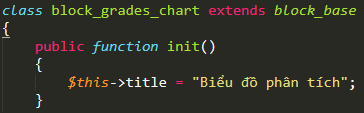
\includegraphics[scale=1]{img/initblock}
		\end{center}
		\caption{Hàm init của Khối}
		\label{refhinh22}
	\end{figure}
\end{center}

\newpage
\subsection{Tệp db/access.php}

Tiếp đến ta tạo tệp access.php nơi cung cấp các quyền truy cập của Khối

\begin{center}
	\begin{figure}[htp]
		\begin{center}
			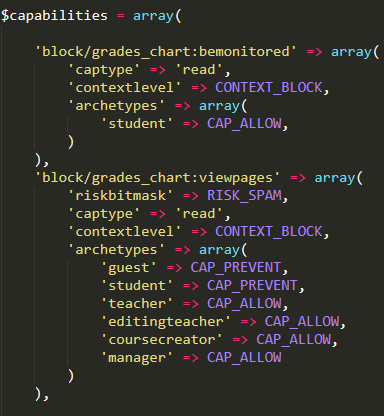
\includegraphics[scale=1]{img/capblock}
		\end{center}
		\caption{Mảng capabilities chứa những quyền truy cập vào Khối}
		\label{refhinh23}
	\end{figure}
\end{center}

\subsection{Tệp lang/en/block\_grades\_chart.php}

Tệp này sẽ chứa ngôn ngữ cho Khối của bạn. Trong phạm vi luận văn nhóm sử dụng tiếng Việt để phát triển cho Khối của mình.

\begin{center}
	\begin{figure}[htp]
		\begin{center}
			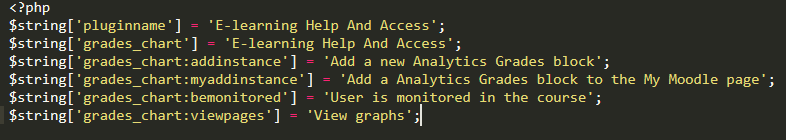
\includegraphics[scale=1]{img/langblock}
		\end{center}
		\caption{Tệp chứa ngôn ngữ cho Khối}
		\label{refhinh24}
	\end{figure}
\end{center}

\newpage
\subsection{Tệp version.php}

Tệp này chứa thông tin của Khối.

\begin{center}
	\begin{figure}[htp]
		\begin{center}
			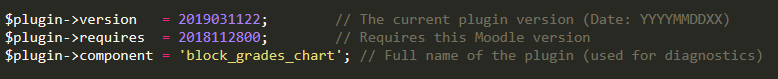
\includegraphics[scale=0.8]{img/in4block}
		\end{center}
		\caption{Thông tin của Khối}
		\label{refhinh25}
	\end{figure}
\end{center}

Trên đây là bốn tệp cơ bản để tạo ra một Khối trong Moodle. Nhưng để Khối hiển thị nội dung ra ngoài màn hình ta cần thêm một phương thức đến lớp của Khối. Code sẽ được thêm vào như sau:

\begin{center}
	\begin{figure}[htp]
		\begin{center}
			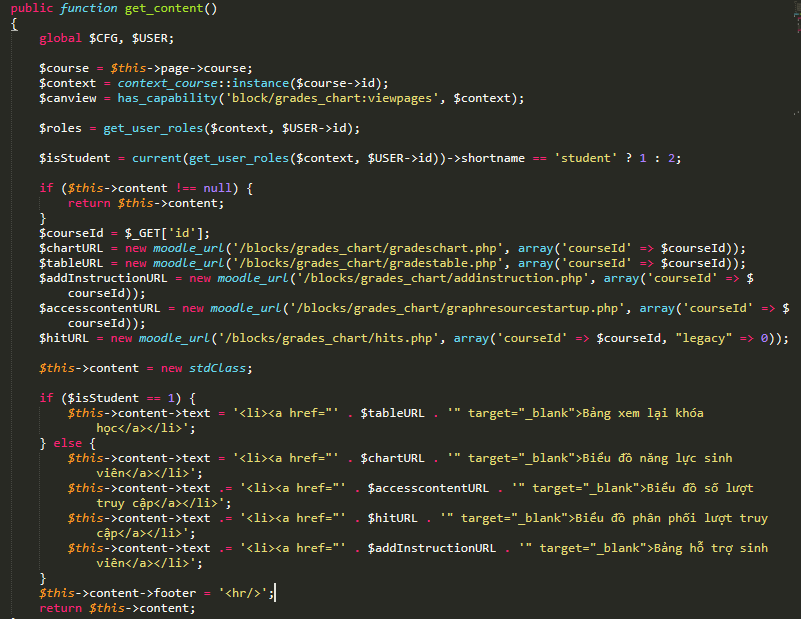
\includegraphics[scale=0.8]{img/contentblock}
		\end{center}
		\caption{Phương thức dùng để hiển thị nội dung của Khối}
		\label{refhinh26}
	\end{figure}
\end{center}

\newpage
\section{Kiến trúc của EHAT}

\begin{center}
	\begin{figure}[htp]
		\begin{center}
			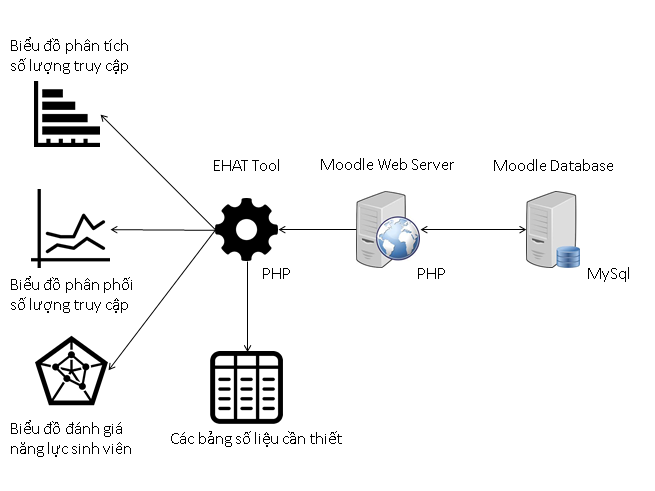
\includegraphics[scale=1]{img/kientrucehat}
		\end{center}
		\caption{Kiến trúc hệ thống EHAT}
		\label{refhinh21}
	\end{figure}
\end{center}

Trên đây là kiến trúc của EHAT trong Moodle. Tiếp đến chúng ta sẽ cùng đi tìm hiểu cách để hiện thực những chức năng của EHAT mà nhóm đã xây dựng.

\section{Hiện thực những chức năng của EHAT}

EHAT là công cụ dễ dàng để sử dụng giúp người dùng phân tích được những dữ liệu trong một khóa học trực tuyến. Bên cạnh đó EHAT còn hỗ trợ cho HV trong quá trình học tập trực tuyến.

Công cụ EHAT hiện nay sẽ hỗ trợ tổng cộng 5 chức năng chính, trong đó 4 chức năng sẽ dành cho GV còn 1 chức năng là của HS,SV. Trước tiên chúng ta sẽ cùng tìm hiểu về 4 chức năng mà EHAT cung cấp cho GV.

\subsection{Đối với GV}

EHAT sẽ cung cấp 4 chức năng chính đối với GV như hình sau:

\begin{center}
	\begin{figure}[htp]
		\begin{center}
			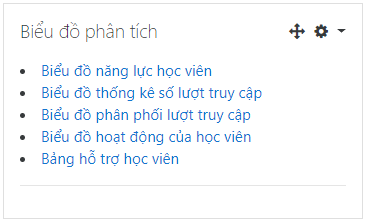
\includegraphics[scale=1]{img/gvtool}
		\end{center}
		\caption{Bốn chức năng mà EHAT mang lại cho GV}
		\label{refhinh27}
	\end{figure}
\end{center}

Trên đây là hình ảnh minh họa 4 chức năng mà EHAT mang lại cho GV, tiếp theo chúng ta sẽ cùng đi vào chi tiết từng chức năng trên xem chúng có gì hay.

\subsubsection{Biểu đồ đánh giá năng lực sinh viên}
Chức năng đầu tiên mà EHAT giành cho GV đó là chức năng đánh giá năng lực sinh viên. Ở chức năng này EHAT sẽ sử dụng biểu đồ mạng nhện(Spider web) để mô tả năng lực của từng cá nhân HV. Kết quả sẽ chỉ ra số điểm trung bình của các tiêu chí mà người dùng tự thiết lập để đánh giá. Bên cạnh đó còn có thêm chức năng so sánh năng lực của hai HV để thấy rõ sự khác biệt về năng lực mỗi cá nhân trong khóa học.

\subsubsection{Biểu đồ thống kê số lượt truy cập}
Để sử dụng chức năng này đầu tiên người dùng phải chọn hạng mục mà mình muốn phân tích số liệu. Ví dụ về các hạng mục mà EHAT hỗ trợ người dùng phân tích:
\begin{itemize}
	\item Bài tập lớn(Assignment)
	\item Trò chuyện(Chat)
	\item Lựa chọn(Choice)
	\item Phản hồi(Feedback)
	\item Diễn đàn(Forum)
	\item Bài giảng(Lesson)
	\item Câu hỏi(Quiz)
	\item Gói SCORM
	\item Khảo sát(Survey)
	\item Wiki
	\item Hội thảo(Workshop)
	\item Sách(Book)
	\item Tài nguyên(Resource)
	\item Tệp tin(Folder)
	\item Trang(Page)
	\item Đường dẫn(URL)
\end{itemize}

Chức năng này cho phép người dùng xem số lượt sinh viên truy cập và không truy cập của từng hạng mục cụ thể mà mình muốn phân tích. Chức năng này giúp GV thấy được mức độ hoạt động của tất cả sinh viên trong khóa học để từ đó có những điều chình phù hợp cho khóa học của mình.

\subsubsection{Biểu đồ phân phối lượt truy cập}
Chức năng sẽ hiển thị cho người dùng một bảng số liệu chứa những thông tin về:
\begin{itemize}
	\item Số lần HV truy cập vào khóa học
	\item Số ngày mà HV truy cập theo tuần kèm biểu đồ mô tả
	\item Số lượng tài nguyên mà HV đã truy cập theo tuần kèm biểu đồ mô tả
\end{itemize}
Bên cạnh đó bảng số liệu cũng có kèm theo dấu hiệu cho thấy HV có thường xuyên truy cập vào khóa học hay không.

\subsubsection{Bảng hỗ trợ sinh viên}
Chức năng cuối cùng mà EHAT hỗ trợ nhằm giúp cho GV thêm tài liệu tham khảo đối với mỗi câu hỏi trong mỗi bài kiểm tra. GV có thể thêm đoạn text hoặc một đường dẫn đến nơi mà mình muốn HV tham khảo. Nội dung sẽ được lưu trữ vào cơ sở dữ liệu và hiển thị cho học viên khi học viên sử dụng chức năng của EHAT.

\subsection{Đối với HS, SV}

Hiện nay EHAT chỉ cung cấp 1 chức năng cho sinh viên:

\subsubsection{Bảng xem lại khóa học}
EHAT hiện chỉ hỗ trợ cho HS, SV chức năng xem lại toàn bộ bài các câu trả lời từ lần làm bài cuối cùng của mình. Trong đó sẽ chỉ rõ câu nào SV trả lời đúng và câu nào SV trả lời sai. Đi kèm với đó là nội dung chi tiết của từng câu hỏi và tài liệu tham khảo nhằm hỗ trợ SV học tập tốt hơn trong quá trình tự học của mình.

\newpage
\section{Đặc tả yêu cầu hệ thống}

\subsection{Yêu cầu chung}

\begin{center}
	\begin{table}[!htp]
		\centering
		\begin{tabular}{|c|c|c|}
			\hline 
			STT & Nội dung & Chi tiết \\ 
			\hline 
			1 & Hệ điều hành & Ubuntu 16.04 \\ 
			\hline 
			2 & Database Server & MySQL  5.6/5.7 \\ 
			\hline 
			3 & Content Server & Apache, >= PHP 7, >= Moodle 3.6 \\ 
			\hline 
		\end{tabular} 
		\caption{Yêu cầu chung của hệ thống}
		\label{bang20}
	\end{table}
\end{center}

\subsection{EHAT đối với GV}
\subsubsection{Biểu đồ đánh giá năng lực sinh viên}
\begin{itemize}
	\item Giới thiệu: Giáo viên có thể đánh giá năng lực của từng cá nhân SV hoặc so sánh 2 SV với nhau.
	\item Inputs
	\begin{itemize}
		\item GV nhập vào số tiêu chí cần thiết lập và chọn nút "Thiết lập".
		\item GV nhập tên các tiêu chí và chọn dữ liệu cho chúng.
		\item GV chọn nút "So sánh" nếu muốn so sánh 2 SV với nhau.
		\item Chọn SV cần phân tích.
		\item Nhấn nút "Xác nhận" để xem biểu đồ.
	\end{itemize}
	\item Quy trình thực hiện
	\begin{itemize}
		\item GV nhấn chọn "Biểu đồ năng lực sinh viên" từ giao diện của Khối EHAT.
		\item GV nhập vào số tiêu chí cần thiết lập và chọn nút "Thiết lập".
		\item GV nhập tên các tiêu chí và chọn dữ liệu cho chúng.
		\item GV chọn nút "So sánh" nếu muốn so sánh 2 SV với nhau.
		\item Chọn SV cần phân tích.
		\item Nhấn nút "Xác nhận" để xem biểu đồ.
	\end{itemize}
	\item Outputs: Giao diện sẽ hiển thị biểu đồ mạng nhện thể hiện năng lực của một sinh viên hoặc so sánh 2 sinh viên mà ta đã chọn để phân tích ở trên.
	\item Xủ lí lỗi
	\begin{itemize}
		\item Nếu GV nhập số tiêu chí ít hơn 3 thì sẽ hiển thị thông báo lỗi và yêu cầu GV nhập lại.
		\item Nếu tên các tiêu chí hoặc dữ liệu của chúng chưa được thêm thì sẽ hiển thị thông báo yêu cầu GV nhập.
		\item Nếu 2 SV so sánh là như nhau thì sẽ hiển thị thông báo lỗi.
	\end{itemize}
\end{itemize}

\subsubsection{Biểu đồ thống kê số lượt truy cập}
\begin{itemize}
	\item Giới thiệu: Giáo viên sử dụng biểu đồ để quan sát số lượng SV tương tác với một hạng mục trong khóa học.
	\item Inputs
	\begin{itemize}
		\item Chọn hạng mục cần tham khảo(Có thể nhấn nút chọn tất cả để xem hết tất cả các hạng mục).
		\item Thiết lập thời gian bắt đầu.
		\item Nhấn nút "Xem biểu đồ" để hiển thị kết quả.
	\end{itemize}
	\item Quy trình thực hiện
	\begin{itemize}
		\item GV nhấn chọn "Biểu đồ thống kê số lượt truy cập" từ giao diện của Khối EHAT
		\item GV sẽ chọn hạng mục cần tham khảo(Có thể nhấn nút chọn tất cả để xem hết tất cả các hạng mục).
		\item GV thiết lập thời gian bắt đầu.(Thời gian mặc định là ngày khóa học bắt đầu).
		\item Nhấn nút "Xem biểu đồ" để hiển thị kết quả.
	\end{itemize}
	\item Outputs: Giao diện sẽ hiển thị biểu đồ cột ngang thể hiện tất cả số lượt truy cập và không truy cập của SV đối với từng hạng mục mà ta đã chọn. Đồng thời hiển thị thêm chi tiết SV nào truy cập hay không truy cập trong hạng mục đó.
	\item Xủ lí lỗi
	\begin{itemize}
		\item Nếu GV không chọn hạng mục thì sẽ hiển thị thông báo lỗi.
	\end{itemize}
\end{itemize}
\subsubsection{Biểu đồ phân phối lượt truy cập}
\begin{itemize}
	\item Giới thiệu: GV dùng để xem xét chi tiết mức độ tương tác của từng cá nhân HS, SV đối với các tài nguyên trong quá trình học.
	\item Inputs: 
	\begin{itemize}
		\item Chọn mục "Biểu đồ phân phối lượt truy cập" từ giao diện của Khối EHAT
		\item Di chuyển chuột vào các điểm trên biểu đồ đường để xem số ngày truy cập trong tuần của sinh viên.
		\item Nhấp vào tên của sinh viên để hiển thị giao diện biểu đồ chi tiết của sinh viên ấy.
		\item Ở giao diện biểu đồ chi tiết của sinh viên chọn mục "Chi tiết lượt truy cập" để xem mức độ tương tác tài nguyên trong khóa học của sinh viên.
		\item Nhấp chọn vùng "Truy cập" để hiển thị biểu đồ chi tiết số lần truy cập của sinh viên đối với các tài nguyên tương ứng
	\end{itemize}
	\item Quy trình thực hiện: Chọn mục "Biểu đồ phân phối lượt truy cập" từ giao diện của Khối EHAT
	\item Outputs: Kết quả sẽ hiển thị bảng số liệu và các biểu đồ tương ứng chứa tất cả thông tin hoạt động của từng cá nhân HS, SV trong khóa học.
	\item Xủ lí lỗi: N/A
\end{itemize}
\subsubsection{Bảng hỗ trợ sinh viên}
\begin{itemize}
	\item Giới thiệu: Giúp GV thêm nguồn tài liệu tham khảo cho HS, SV.
	\item Inputs
	\begin{itemize}
		\item GV chọn nút "Thêm hướng dẫn".
		\item GV chọn câu hỏi cần thêm tham khảo và nhập nội dung tham khảo vào câu hỏi đó.
		\item Nhấn nút "Xác nhận" để thêm tài liệu tham khảo.
	\end{itemize}
	\item Quy trình thực hiện
	\begin{itemize}
		\item GV nhấn chọn "Bảng hỗ trợ sinh viên" từ giao diện của Khối EHAT
		\item GV chọn nút "Thêm hướng dẫn".
		\item GV chọn câu hỏi cần thêm tham khảo và nhập nội dung tham khảo vào câu hỏi đó.
		\item Nhấn nút "Xác nhận" để thêm tài liệu tham khảo.
	\end{itemize}
	\item Outputs: Nội dung tham khảo sẽ được thêm vào database để hỗ trợ SV.
	\item Xủ lí lỗi: N/A
\end{itemize}

\subsection{EHAT đối với HS, SV}
\subsubsection{Bảng xem lại khóa học}
\begin{itemize}
	\item Giới thiệu: Giúp SV xem lại kết quả của các bài kiểm tra của mình trong khóa học.
	\item Inputs: SV nhấn chọn "Bảng xem lại khóa học" từ giao diện của Khối EHAT
	\item Quy trình thực hiện: SV nhấn chọn "Bảng xem lại khóa học" từ giao diện của Khối EHAT
	\item Outputs: Công cụ sẽ hiển thị ra bảng kết quả chứa tất cả thông tin về câu trả lời của SV trong quá trình kiểm tra.
	\item Xủ lí lỗi: N/A
\end{itemize}